\marginnote{Beginning of parsing.tex}

Given a grammar model and a curve, we want to calculate how likely the
curve is under the model, and we would like to extract the most likely
correspondence between the points of the curve and the parts of the
model. We call this process parsing, because it is extremely similar
to CKY parsing with standard PCFG's. We defer the technical details of
parsing until a later chapter.

We examine parsing in this section by looking at human silhouettes
from the Romer dataset. We have two versions of this dataset: one
where a silhouette has been automatically extracted by subtracting the
background, and the curve simplified slightly by the discretization
method discussed in Section \ref{sec-models-curves}; and a
hand-annotated version, where we have marked by hand the position of
27 corresponding points on the body in each image. 

Throughout this section, we examine the task of building a grammatical
model from one curve, and using it to parse another curve. We
demonstrate the accuracy of these parses by showing the correspondence
between the points of the two curves induced by the most likely parse.

The easiest parsing task is to recover a one-to-one correspondence
between two curves that have the same number of points, which we
demonstrate in Figure \ref{fig-one-to-one}. Because there are no
missing or extra points, this is straightforward.  The two curves are
both from the hand-annotated Romer dataset. The grammar is built using
a hand-picked set of constituents.

\begin{figure}
\includegraphics[width=\linewidth]{output/2.parsing/one_to_one/parse.png}
\caption{Recovering a One-to-one Correspondence}
\label{fig-one-to-one}
\end{figure}

A somewhat harder task is to parse a curve that is longer than the
curve on which our model is based. We wish to recover a reasonable
correspondence between the points of the coarse model curve and a
subset of the points of the finer input curve. We do this by building
a grammar model from the coarse curve and using it to parse the finer
curve. The grammar must have lengthening rules, but doesn't need
shortening rules. This demonstrates that we can model longer curves
than were used to build the grammar. This is shown in Figure
\ref{fig-longer}, where a model built from a hand-annotated curve is
used to parse a curve from the ground-truth Romer dataset. We
successfully recover a very reasonable correspondence.

\begin{figure}
\includegraphics[width=\linewidth]{output/2.parsing/longer_curves/parse.png}
\caption{Parsing a Longer Curve}
\label{fig-longer}
\end{figure}

We also wish to recover a reasonable correspondence by building a
grammar from a longer (i.e., finer) model curve and parsing a shorter
(i.e., coarser) input curve. This demonstrates that we can model
shorter curves than were used to build the grammar. This task is
generally harder than the prior task.

Here we build a grammar from a ground-truth Romer curve, and try to
parse one of the (much shorter) hand-annotated Romer curves. We can
safely assume that every point in the parsed curve has a corresponding
one in the example curve, which is the reverse of the previous
experiments. In order to do this successfully, the grammar needs
shortening rules, but not lengthening rules.

In Figure \ref{fig-shorter-1}, we show the results of parsing a
shorter curve with very little geometric variation. The fine details
are not quite right, but overall the correspondence is reasonable. In
Figure \ref{fig-shorter-2}, we show the results of parsing a shorter
curve with significant geometric variation. In this case, the
correspondence found is completely incorrect.

Our models are very sensitive to the initial decomposition specified
for the model curve. The two experiments above used a balanced but
otherwise arbitrary decomposition of the model curve. By using a more
carefully chosen decomposition, we get much better parses, which can
be seen in Figures \ref{fig-shorter-3} and \ref{fig-shorter-4}. In
Figure \ref{fig-shorter-3}, the fine details are now exactly what we
would expect, in contrast to Figure \ref{fig-shorter-1}. In Figure
\ref{fig-shorter-4}, even though we have the same significant
geometric variation as in Figure \ref{fig-shorter-2}, we now find a
very good correspondence.

\begin{figure}
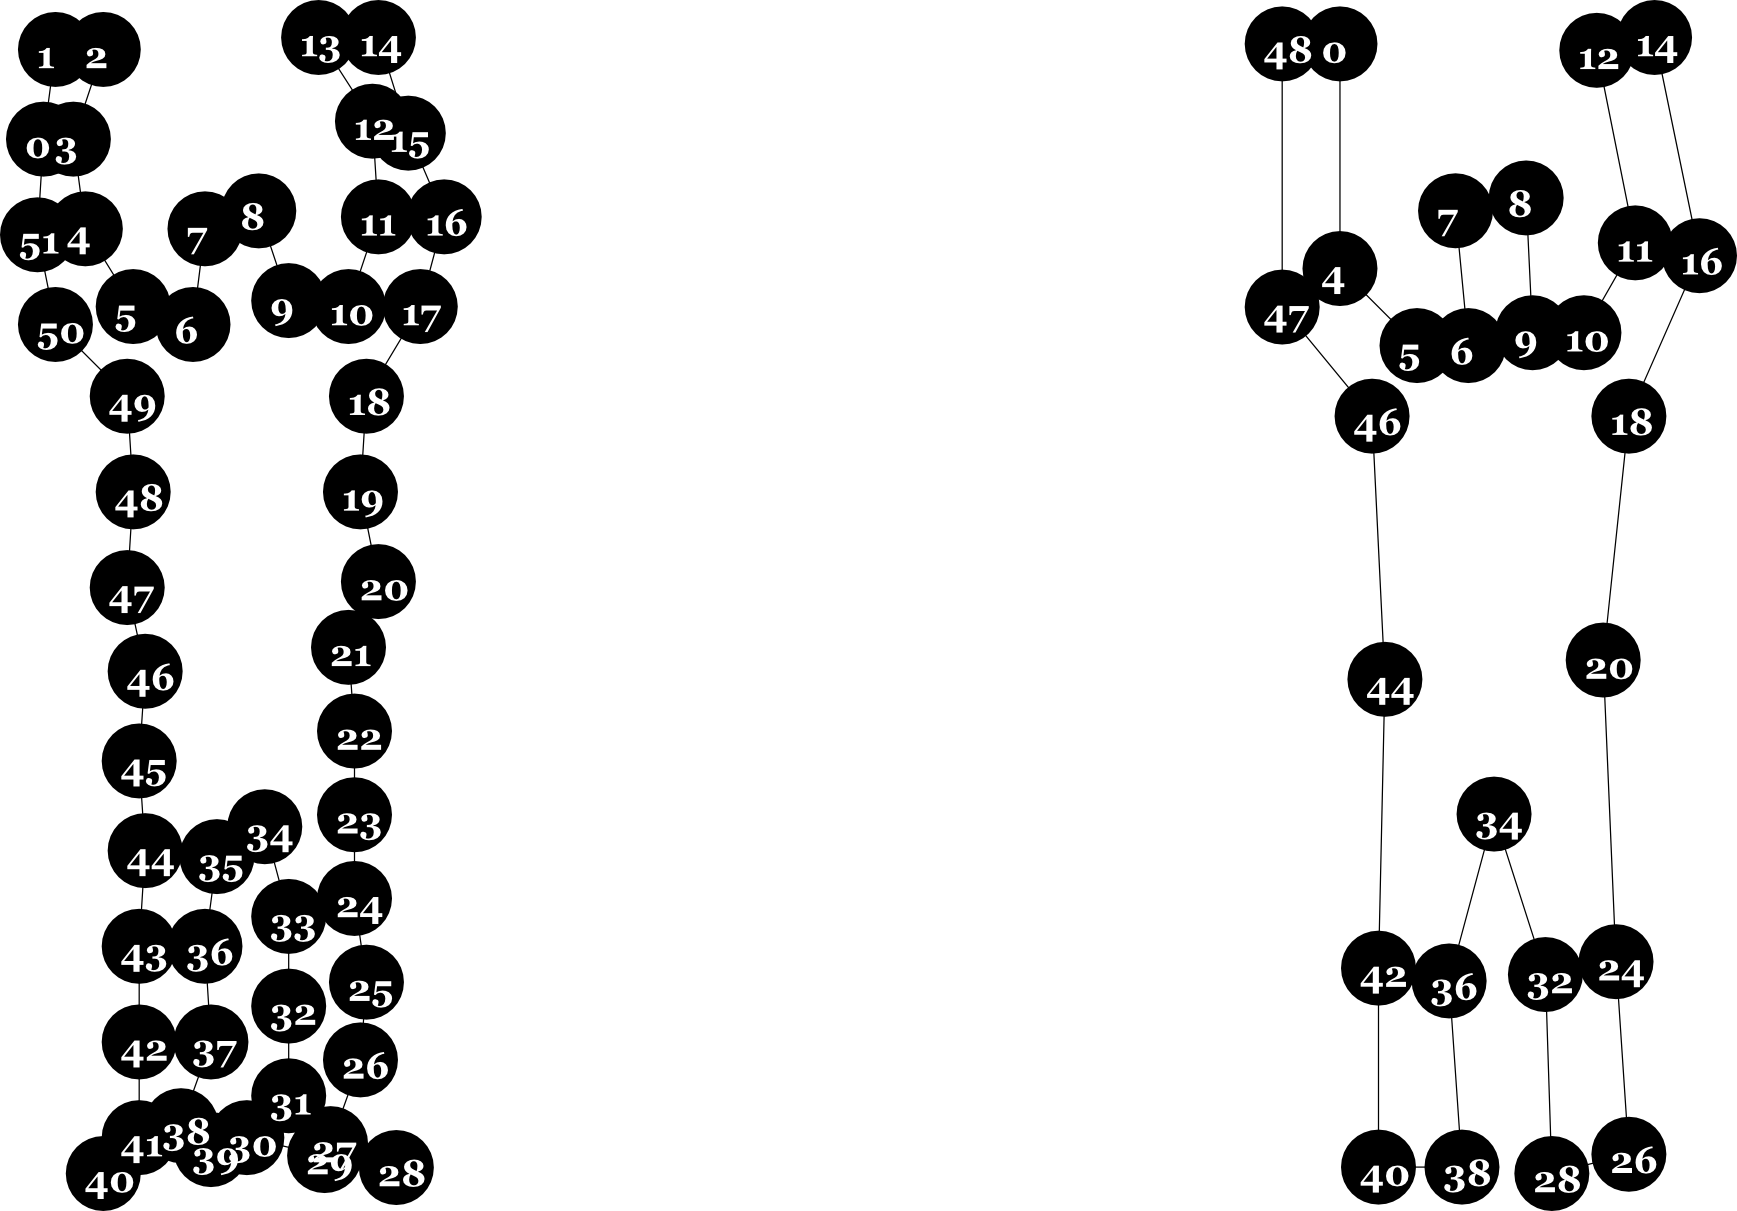
\includegraphics[width=\linewidth]{output/2.parsing/shorter_curves/parse_8.png}
\caption{Parsing a shorter curve with very little geometric variation.}
\label{fig-shorter-1}
\end{figure}

\begin{figure}
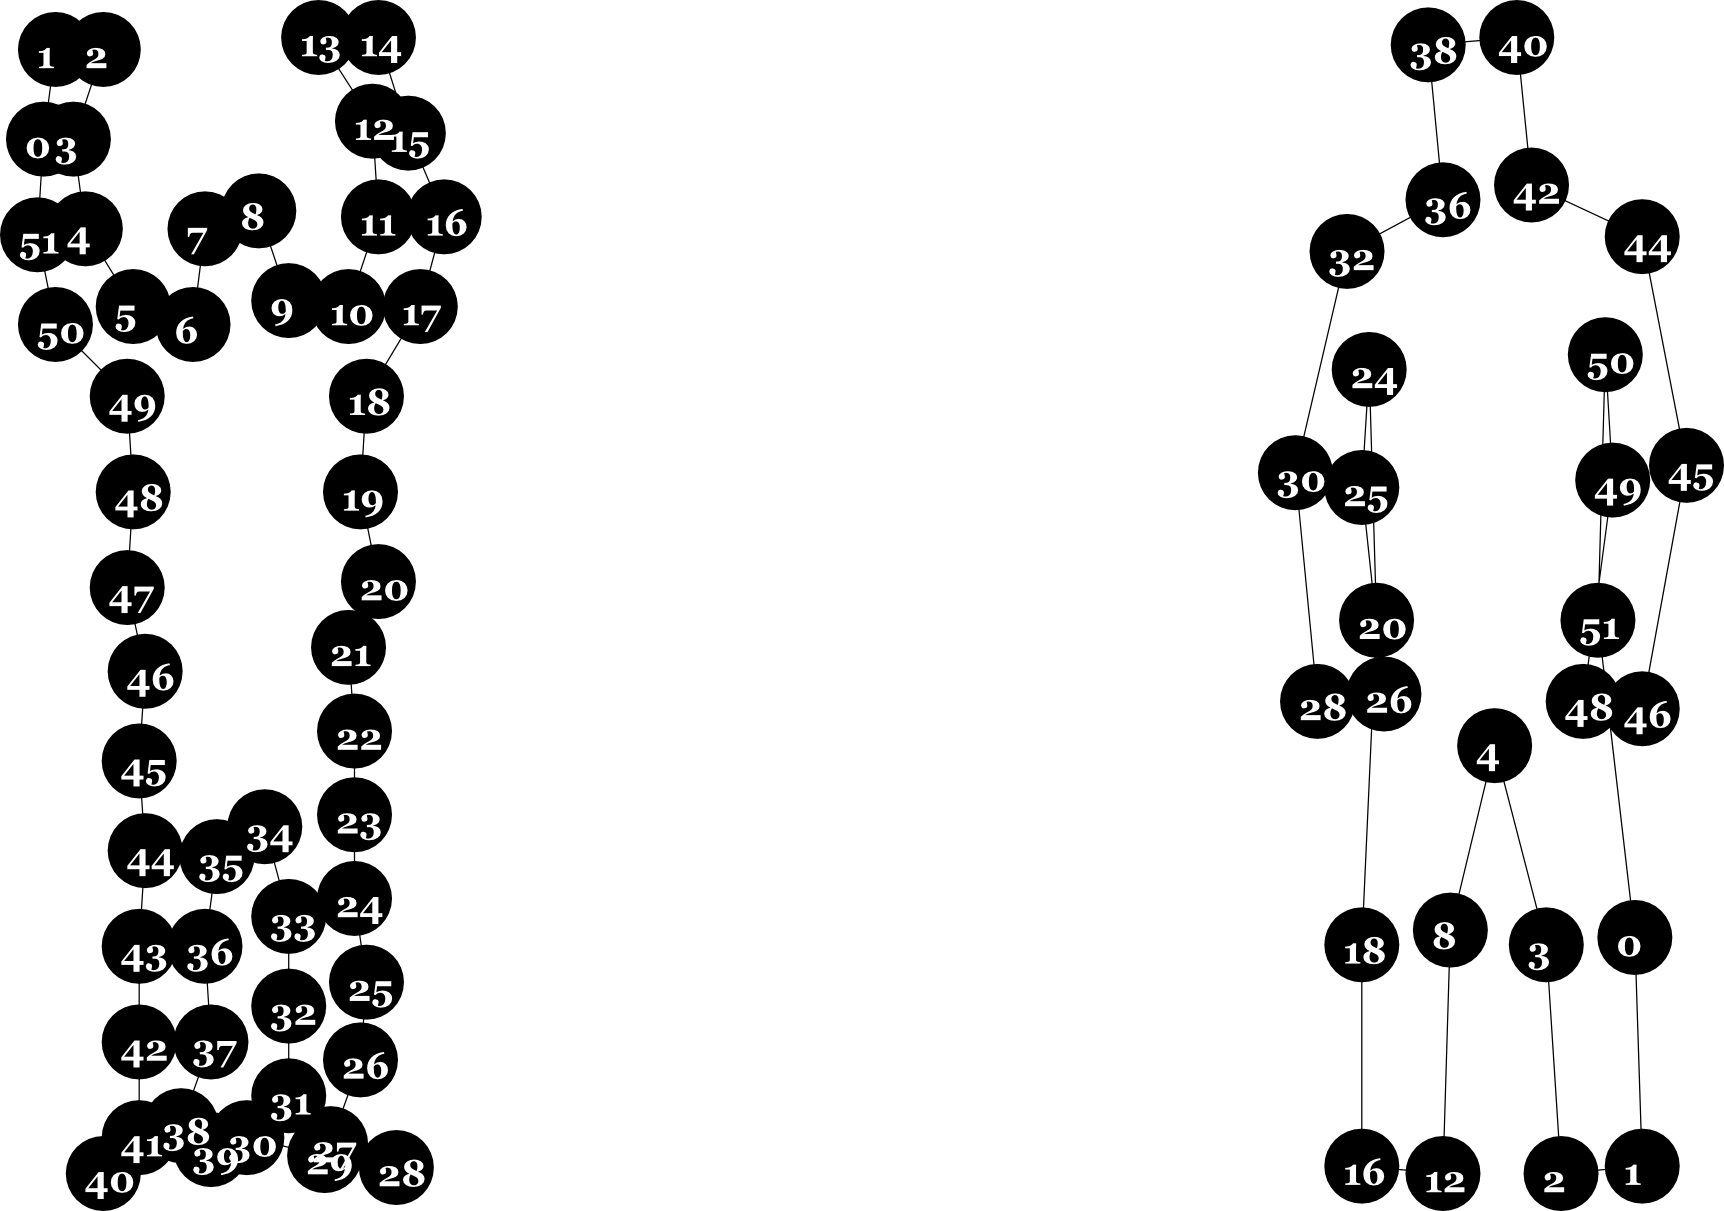
\includegraphics[width=\linewidth]{output/2.parsing/shorter_curves/parse_0.png}
\caption{Parsing a shorter curve with significant geometric
  variation. }
\label{fig-shorter-2}
\end{figure}

\begin{figure}
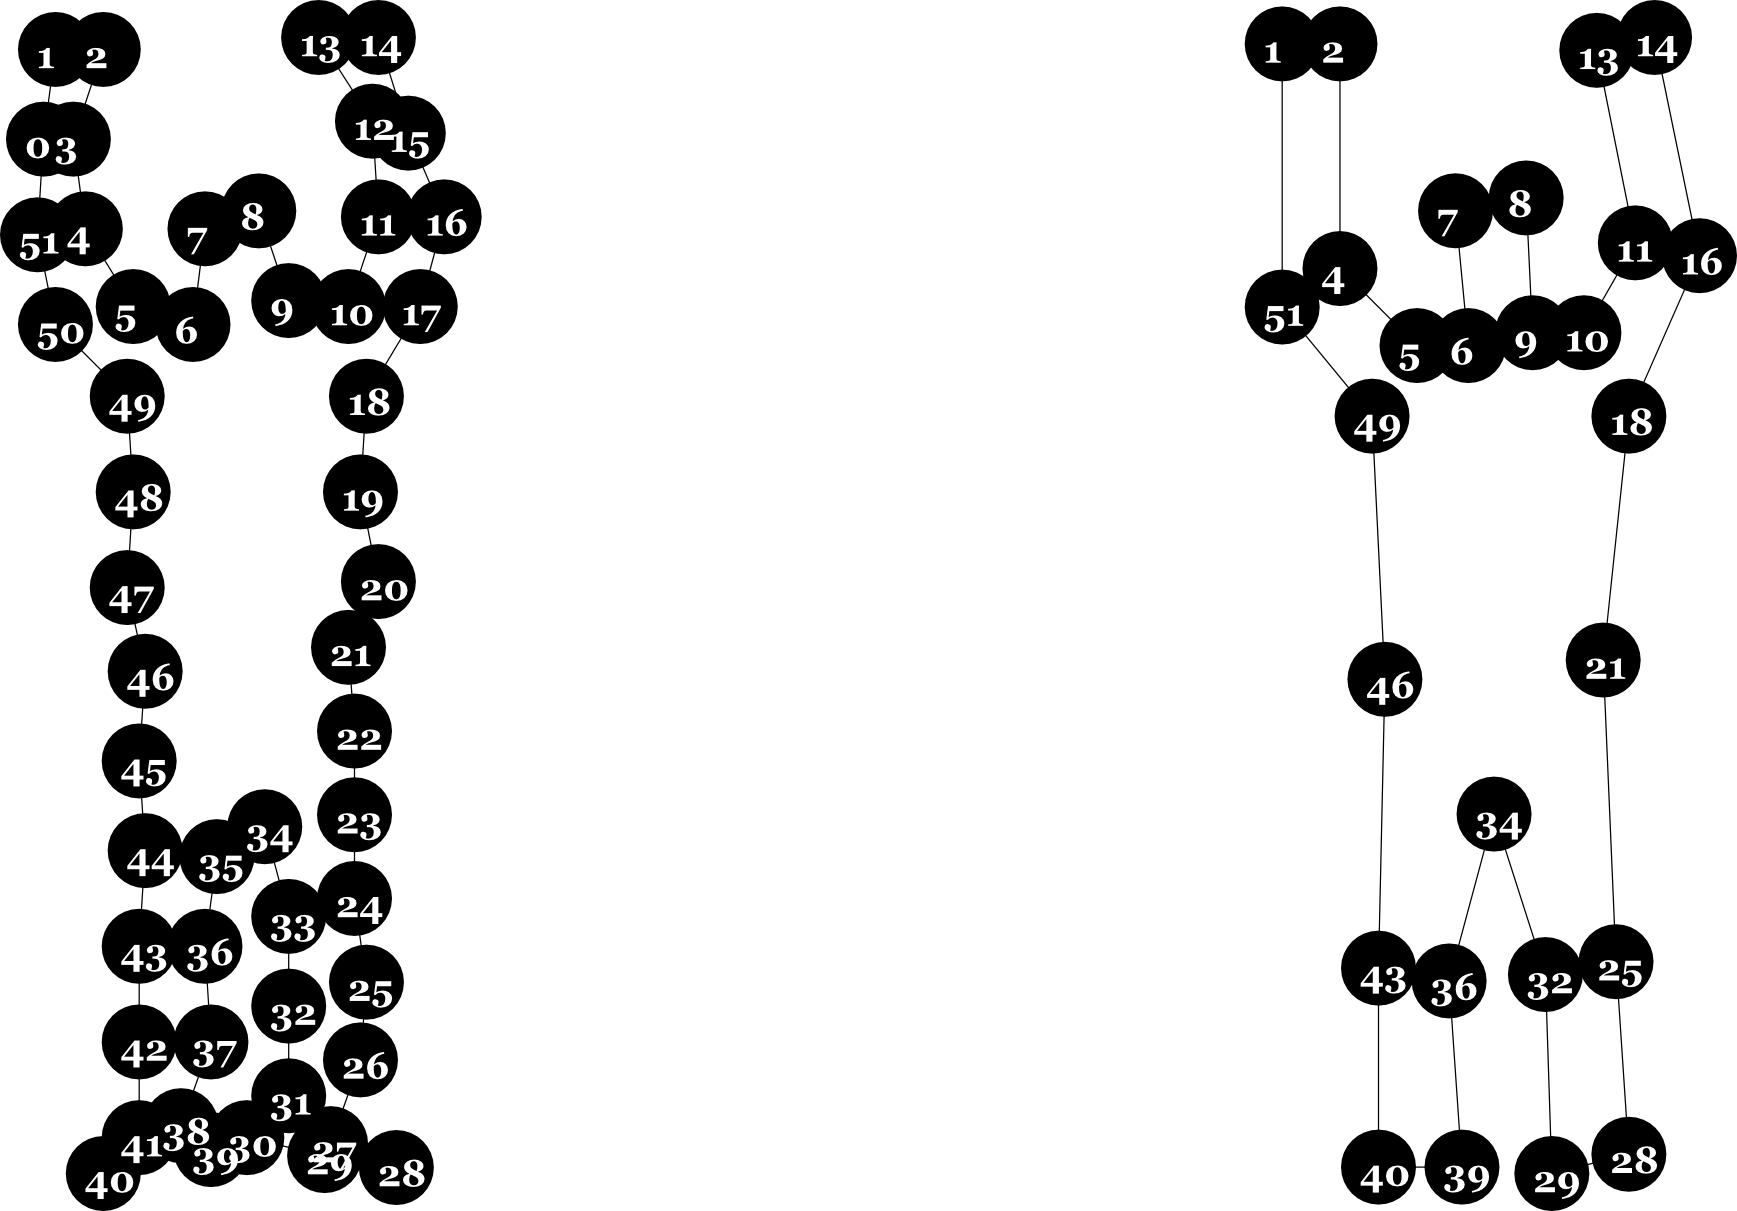
\includegraphics[width=\linewidth]{output/2.parsing/shorter_curves/parse_8_2.png}
\caption{Parsing a shorter curve with very little geometric
  variation.}
\label{fig-shorter-3}
\end{figure}

\begin{figure}
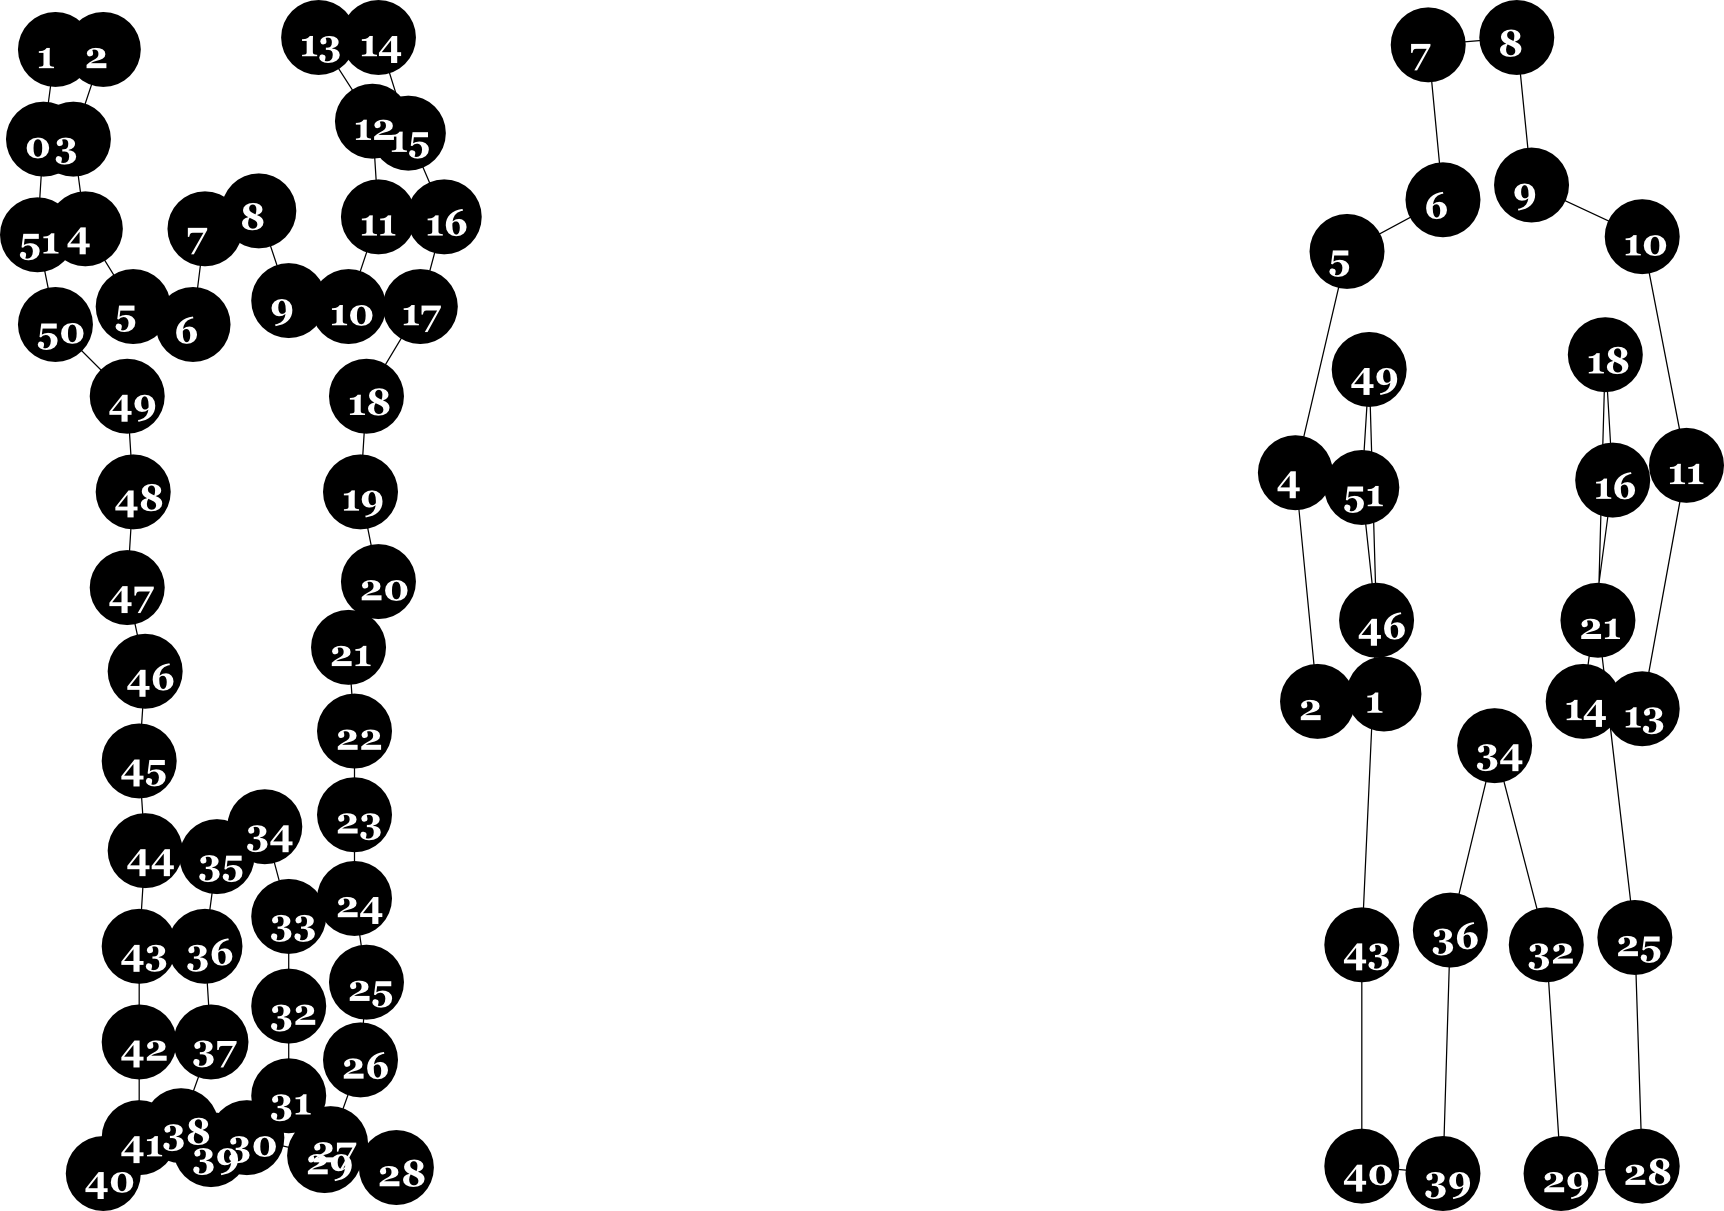
\includegraphics[width=\linewidth]{output/2.parsing/shorter_curves/parse_0_2.png}
\caption{Parsing a shorter curve with significant geometric
  variation.}
\label{fig-shorter-4}
\end{figure}

\FloatBarrier

Thus, even on fairly straightforward parsing tasks, our models are
extremely sensitive to the particular structure that we impose on the
curve. The shortening rules only allow the parser to chop off
constituents. If the constituents look bad, then the parse will look
bad.

%%

\marginnote{Given a coarse curve and a finer curve, where the finer curve has
    features not present in the coarse curve (such as bumps or pits),
    recover a reasonable correspondence by building a grammar from the
    coarse curve and using it to parse the finer curve. This
    demonstrates that we can model longer curves that have non-trivial
    variation in detail.}

\marginnote{Given two fine curves which do not have a perfect correspondence,
    recover a reasonable correspondence by building a grammar from one
    and using it to parse the other. This demonstrates that we can
    model both extra and missing points.}


\marginnote{End of parsing.tex}

